\subsection{Experiment 5: Enhancing Performance with Regularization Techniques} \label{sec:exp5}

In this experiment, the author aimed to test the hypothesis that incorporating regularization techniques can enhance model performance. As such, several regularization techniques were utilized in the model. Initially, dropout layers were added, which randomly deactivate a percentage of neurons during training. This technique strengthens the model's ability to generalize. Batch normalization was included to normalize layer activations and decrease internal covariate shifts, speeding up training.

Additionally, the author introduced noise to the discriminator input to enhance model robustness, making it less sensitive to small perturbations and improving overall stability. Elastic network regularization, which combines both L1 and L2 penalties, was also utilized~\cite{zou_regularization_2005}.

It should be noted that the experimental setup was identical to Experiment 4, except for the use of the Adam optimizer. The total loss for this experiment was $4.791$, calculated by summing the generator loss of $3.362$ and the discriminator loss of $1.428$. However, it is important to note that comparing the current generator loss to previous results is not appropriate due to the incorporation of the elastic net regularization. This regularization method substantially elevates the generator loss but is crucial for training goals.

Regrettably, a flaw in the elastic net implementation was detected in the code, but not until after a few subsequent experiments. Although this error has a negative impact on the overall absolute loss and results, it does not affect the comparisons between experiments.

Refer to Figure~\ref{fig:exp5_results} for a visual representation of the results, displaying the loss and final spectrogram generated in this experiment.

\begin{figure}[!ht]
    \centering
    \begin{subfigure}{0.45\textwidth}
        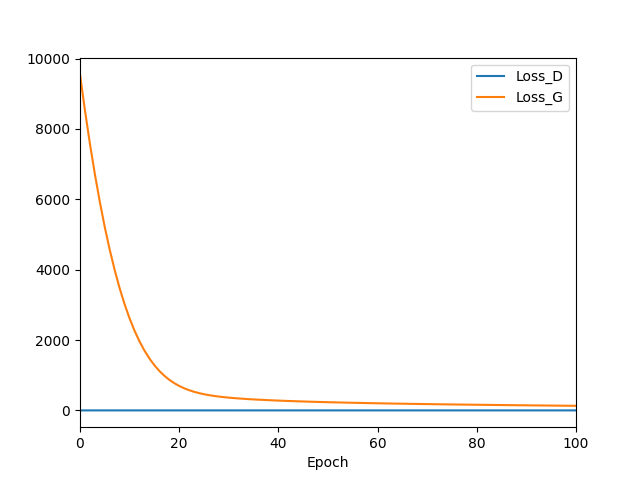
\includegraphics[width=\textwidth]{figures/4.5-results/exp5_loss.png}
        \caption{Evolving losses throughout the training process for Experiment 5.}
        \label{fig:exp5_loss}
    \end{subfigure}
    \begin{subfigure}{0.45\textwidth}
        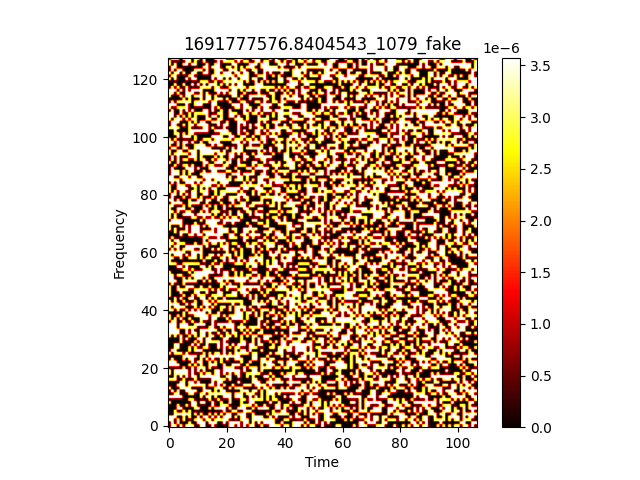
\includegraphics[width=\textwidth]{figures/4.5-results/exp5_spectrogram.png}
        \caption{Spectrogram generated in Experiment 5.}
        \label{fig:exp5_spectrogram}
    \end{subfigure}
    \caption{Results of Experiment 5.}
    \label{fig:exp5_results}
\end{figure}